\section{Soft Divergences II}

\subsection{1-Loop correction to $e^+e^- \to \mu^+\mu^-$, continued}
We were computing the 1-loop correction to the $e^+e^- \to \mu^+\mu^-$ cross section:

\begin{center}
    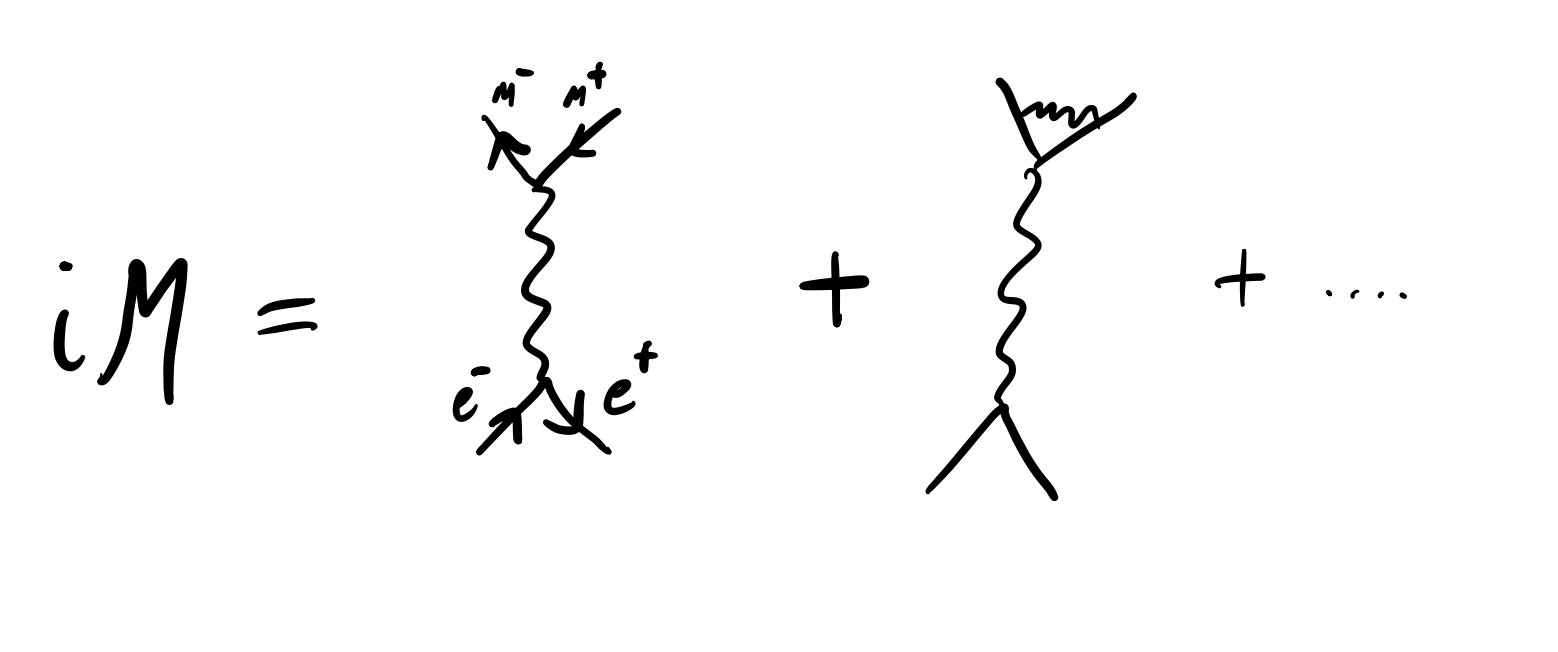
\includegraphics[scale=0.35]{Lectures/Images/lec15-1loopdiagrams.png}
\end{center}

where we found:
\begin{equation}
    i\mathcal{M} = \frac{ie^2}{s}(\bar{v}_2\gamma^\rho u_1)(\bar{u}_3(\gamma_\rho + \Gamma_\rho)v_4)
\end{equation}
with:
\begin{equation}
    \Gamma_\rho = \left.\avg{j_\rho(p_3 + p_4)\psi\bar{\psi}(-p_4)}_{\text{amp}}\right|_{\text{1-loop}} = \gamma_\rho \frac{e^2}{8\pi^2}\int_0^1 dx\int_0^{1-x}dy \frac{s}{\Delta}
\end{equation}
with:
\begin{equation}
    \begin{split}
        \Delta = m_\gamma^2(1 - x - y) - (xp_3 - yp_4)^2 &= m_\gamma^2(1-x-y) + (x^2 + y^2)M^2 + 2p_3 \cdot p_4xy
        \\ &\approx m_\gamma^2(1-x-y) + 2p_3 \cdot p_4xy
        \\ &= m_\gamma^2(1 - x - y) - sxy
    \end{split}
\end{equation}
where we focus on high $E$ ($E \gg M$) scattering in the second-to-last line, and in the last line we use the approximate expression for the Mandelstam variable:
\begin{equation}
    s = -(p_3 + p_4)^2 = 2M^2 - 2p_3 \cdot p_4 \approx -2p_3 \cdot p_4
\end{equation}
Let's look at these final two integrals. They will do something unusual. They can be computed exactly (as you will see on PS8), and the leading $m_\gamma \to 0$ singularity is:
\begin{equation}
    \int_{xy}\frac{s}{\Delta} \approx -\frac{1}{2}(\log \frac{m_\gamma^2}{s})^2 \implies \Gamma_\rho = -\gamma_\rho\frac{e^2}{16\pi^2}(\log\frac{m_\gamma^2}{s})^2
\end{equation}
this is quite unusual. These logarithms are called the Sudhakov double-logarithm. They are unlike what we saw in RG, which were logarithms which we were able to resum.

Let's sketch the computation of this integral. If we send $m_\gamma^2 \to 0$, $\frac{1}{\Delta}$ becomes singular for $x \to 0$ or $y \to 0$. Let's take a look at these regions:
\begin{equation}
    \begin{split}
        \int_{xy}\frac{s}{\Delta} = \int_0^1 dx \int_0^{1-x}dy \frac{1}{\frac{m_\gamma^2}{s}(1-x-y) - xy} &\sim \int_0^1 dx \int_0^1 dy \frac{1}{\frac{m_\gamma^2}{s} - xy} 
        \\ &= \int_0^1dx \frac{1}{x}\left.\log(\frac{m_\gamma^2}{s} - xy)\right|_0^1
        \\ &= \int_0^1 dx \frac{1}{x}\left[\log(\frac{m_\gamma^2}{s} - x) - \log\frac{m_\gamma^2}{s}\right] 
        \\ &= \int_0^1 dx \frac{1}{x}\log(1 - \frac{s}{m_\gamma^2}x)
    \end{split}
\end{equation}
Now using the identity that $\dod{}{z}\frac{1}{2}\log^2(z) = \frac{\log z}{z}$ we find that the above integral evaluates to $\sim \frac{1}{2}\log^2$.

Hence, our matrix element becomes:
\begin{equation}
    i(\mathcal{M} + \mathcal{M}_\Gamma) = \frac{ie^2}{s}(\bar{v}_2\gamma^\rho u_1)(\bar{u}_3\gamma_\rho v_4)\left[1 - \frac{e^2}{16\pi^2}\left(\log\frac{m_\gamma^2}{s}\right)^2 + \ldots\right]
\end{equation}
where - nicely - the spins structure is exactly the same! So whatever we did for the tree level piece carries over. We thus find that:
\begin{equation}
    \sigma(e^+e^- \to \mu^+\mu^-) = \int \frac{1}{4}\sum_s \abs{\mathcal{M}}^2 d\Pi_{\text{LIPS}} = \frac{e^4}{12\pi s}\left[1 - \ldots\right]^2 = \frac{e^4}{12\pi s}\left[1 - \frac{e^2}{8\pi^2}\left(\log\frac{m_\gamma^2}{s}\right)^2 + \ldots\right]
\end{equation}

\subsection{Real emission processes}
Clearly this cross section doesn't make sense. It involves an unphysical parameter, and if we send $m_\gamma^2 \to 0$ it diverges. So it can't possibly be the final answer to anything physical. But what we noticed last week is that there are other types of diagrams involving soft photons (that we would usually associate to different scattering events) that had the same dependence on parameters/charges. We may have hope that these extra processes - known as real emission processes - may help us out here, and cancel out the IR divergences. Let us thus study an ``inclusive'' cross-section that includes these soft photons. Thus:
\begin{equation}
    \sigma_{\text{tot}} = \sigma(e^+e^- \to \mu^+\mu^-) + \sigma(e^+e^- \to \mu^+\mu^-\gamma) + \ldots
\end{equation}
where we only need to consider one soft photon as at this order we have the $\sigma \sim e^6$/same order.

\begin{center}
    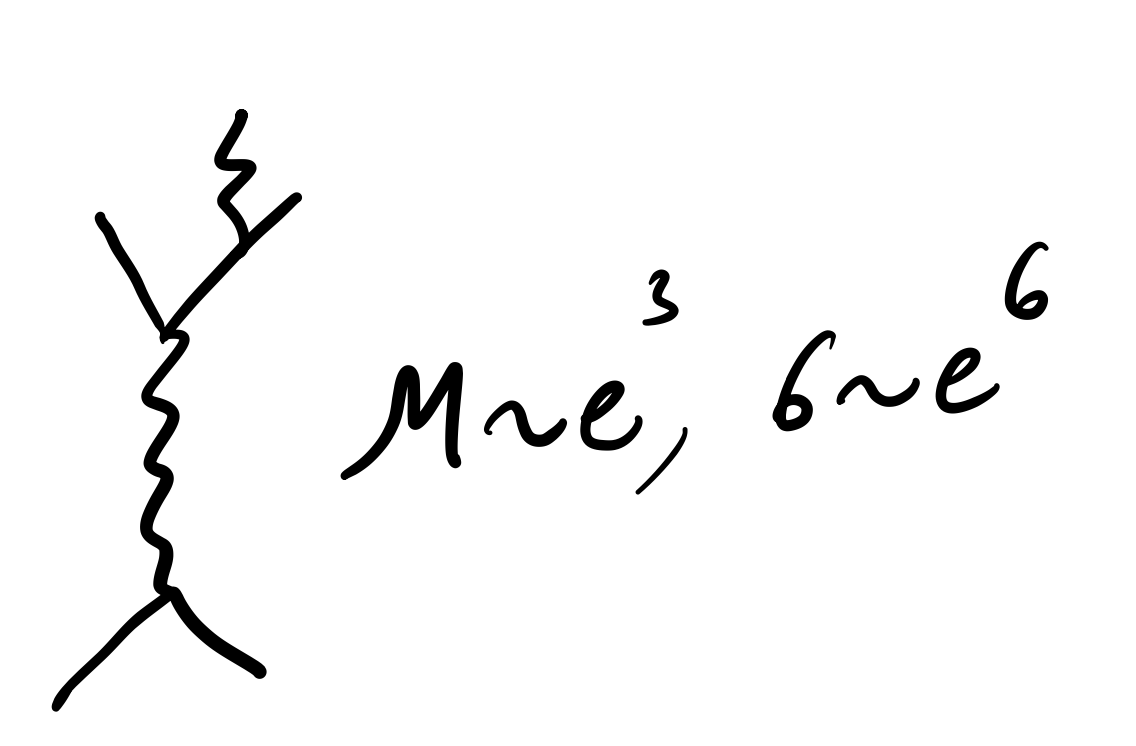
\includegraphics[scale=0.35]{Lectures/Images/lec15-eorder.png}
\end{center}

Let's draw the two relevant diagrams for $e^+e^- \to \mu^+\mu^-\gamma$, where we have a soft photon emitted from the muon.

\begin{center}
    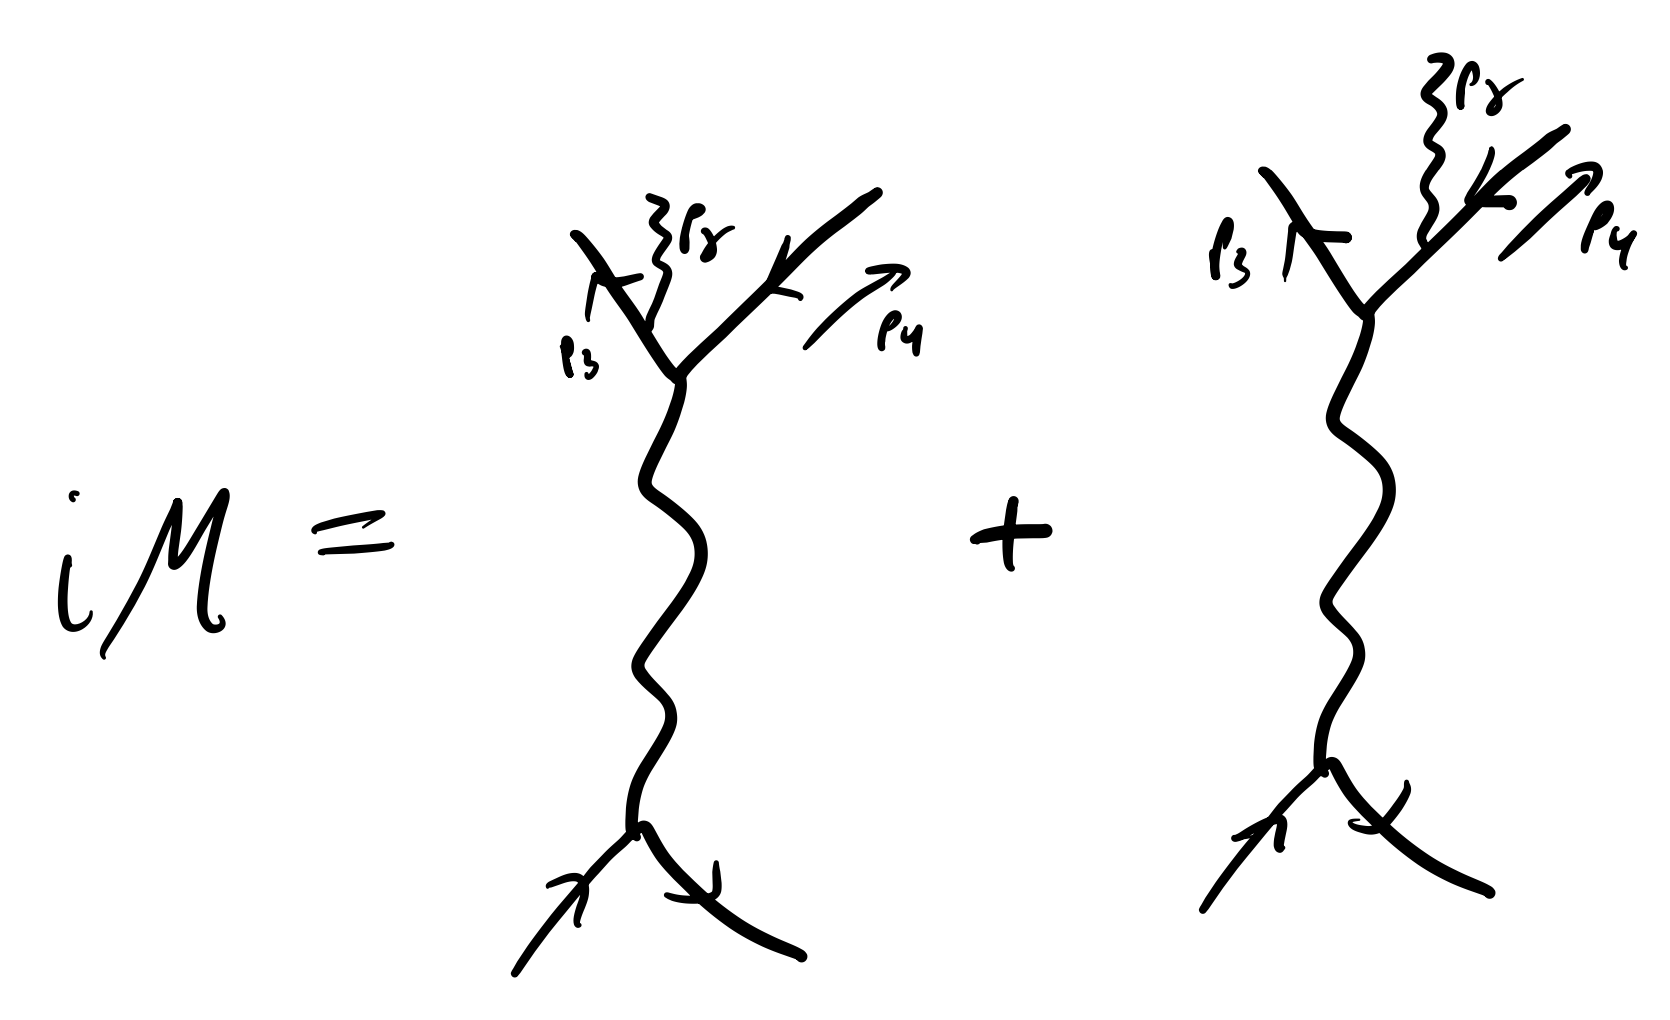
\includegraphics[scale=0.35]{Lectures/Images/lec15-softphotons.png}
\end{center}

These are just tree-level diagrams with no integrals. Where do the divergences come from? The intuition is that we had a singular result in the no-photon case because our detector was insensitive to emitted photons. For the photon cross-section, we need to integrate over all photon momenta $\int \frac{d^3\v{p}_\gamma}{(2\pi)2\e_\gamma}$ - this indeed has a chance of introducing singularities.

The full derivation is tedious, and is in Schwarz Ch. 20 for your reference. Let's start with the nontrivial key step (which is one of the final ones). We have matrix element:
\begin{equation}
    \mathcal{M} \sim \frac{1}{s}\frac{1}{p_4\cdot p_\gamma}
\end{equation}
where the $\frac{1}{s}$ comes from the photon propagator and the $\frac{1}{p_4 \cdot p_\gamma}$ comes from the Dirac propagator. The square of this gives:
\begin{equation}
    \mathcal{M}^2 \sim \frac{1}{s^2}\frac{1}{(p_4 \cdot p_\gamma)^2}
\end{equation}
To get the cross section, we integrate:
\begin{equation}
    \sigma \sim \int d\Pi_{\text{LIPS}}\abs{\mathcal{M}}^2
\end{equation}
so let us integrate over the photon phase space $d^3p_\gamma$. Say we choose our coordinate system such that $p_4 = (E, 0, 0, E)$. We can then take:
\begin{equation}
    \v{p}_\gamma = p_\gamma(\cos\theta\zhat + \sin\theta\xhat)
\end{equation}
with the $\phi$-integral giving $2\pi$. 

\begin{center}
    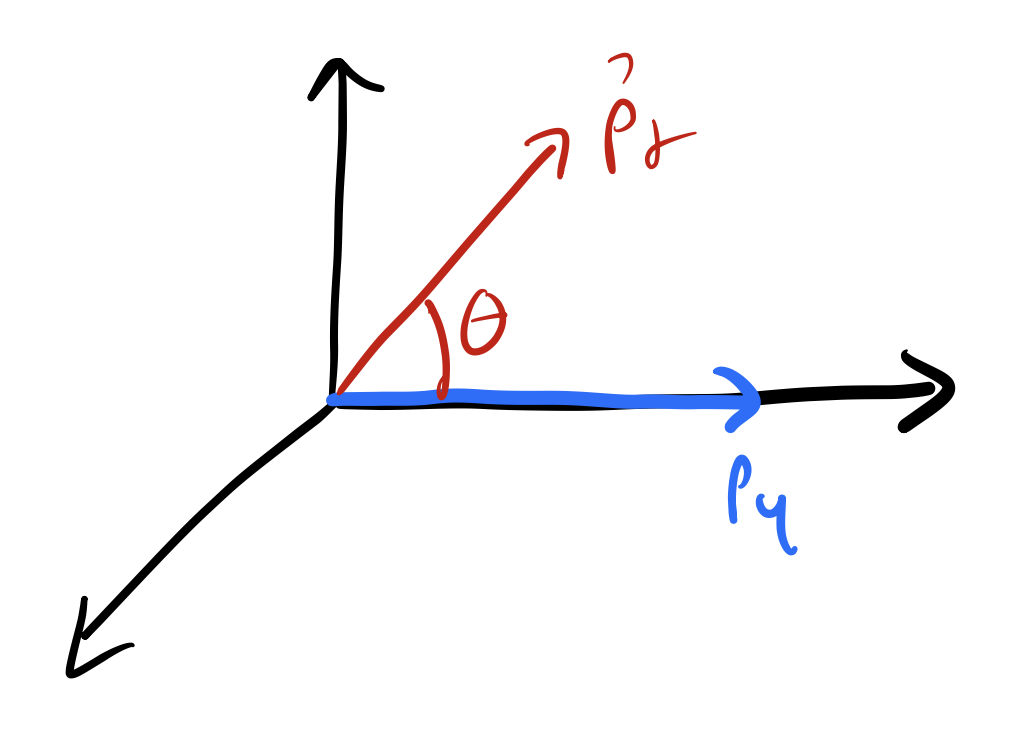
\includegraphics[scale=0.35]{Lectures/Images/lec15-angles.png}
\end{center}

Putting the photon on-shell, the 0th component is given by;
\begin{equation}
    p^0_\gamma = \sqrt{\v{p}_\gamma^2 + m_\gamma^2} = \e_p^\gamma
\end{equation}
So then:
\begin{equation}
    p_4 \cdot p_\gamma = E(\sqrt{\v{p}_\gamma^2 + m_\gamma^2} + p_\gamma\cos\theta)
\end{equation}
So then the integral gives:
\begin{equation}
    \sigma \sim \int \frac{d^3\v{p}_\gamma}{(2\pi)^32\e_p^\gamma}\abs{\mathcal{M}}^2 \sim \int_{-1}^1 d\cos\theta \int \frac{dp_\gamma p_\gamma^2}{(\sqrt{p_\gamma^2 + m_\gamma^2} + p_\gamma\cos\theta)^2\cdot\sqrt{p_\gamma^2 + m_\gamma^2}}
\end{equation}
Which if $m_\gamma \to 0 $ then we get $\int \frac{dp_\gamma}{p_\gamma} \sim \log m_\gamma^2$, with if we did the two integrals carefully, we would get $(\log m_\gamma^2)^2$. Hence we will see the divergences cancel out.\footnote{Though we didn't compute the finite part/the important part of the 1-loop correction, we certainly could have, and we would see that the infinities/IR divergences cancel while the finite part persists.}

\subsection{Cross section with soft photons, more carefully}
From the two diagrams with soft photons, we compute:
\begin{equation}
    i\mathcal{M} = \avg{\mathcal{T}A_\mu(p_\gamma)\bar{\psi}_a(p_4)\psi_c(p_3)\psi_b(p_2)\bar{\psi}_a(p_1)}_c
\end{equation}
Now the various fields in this diagram become: $[\bar{v}_2(-\slashed{p}_2 + m)]_b$ (and other relevant $v/u$ for the fermion fields), and $e_\mu^{(h)}p_\gamma^2$ for the photon helicity.

To construct the relevant diagrams with three vertices, we will insert $\frac{i^3}{3!}(S_{\text{int}})^3$ and contract with various places. The $\frac{1}{3!}$ cancels with combinatorics, and we are left with:
\begin{equation}
    \avg{\ldots}_c = (ie)^3\avg{A_\mu(p_\gamma)\int A_\lambda \bar{\psi}\gamma^\nu\psi \left(\int A_\rho \bar{\psi}\gamma^\rho \psi\right) \bar{\psi}_d(p_4)\psi_c(p_3)\psi_b(p_2)\bar{\psi}_a(p_1)\int A_\lambda \bar{\psi}\gamma^\lambda \psi}
\end{equation}
where we can now contract the electro fields. The external photon and electron propagators cancel in the LSZ formula, so we find:
\begin{equation}
    i\mathcal{M} = i^2\e^{(h)}_\nu[\bar{u}_3(\slashed{p}_3 + M)]_c[(-\slashed{p}_4 + M)v_4]_d (\bar{v}_2\gamma^\lambda u_1) \cdot (ie)^3\avg{(\bar{\psi}\gamma^\nu \psi)(p_\gamma)\bar{\psi}_d(p_4)\psi_c(p_3)\left(\int A_\rho \bar{\psi}\gamma^\rho \psi\right)A_\lambda(p_1 + p_2)}
\end{equation}
Now we can contract the last two remaining photon fields. Further, we can contract $\psi_c(p_3)$ with the $\bar{\psi}$ of the soft photon, $\psi$ of the $p_\gamma$ contracts with the rest of the vertex, and and the remaining $\psi$ contracts with $\bar{\psi}_d(p_4)$. Each of these gives a minus sign (three minus signs, so leads to $-1$). Option 2 is to contract $\bar{\psi}_d(p_4)$ with the soft photon vertex. You can work it out to see that this also gives $-1$. Writing this out, we obtain:
\begin{equation}
    \begin{split}
        i\mathcal{M} &= i\e^{(h)}_\nu e^3\left(\bar{u}_3\gamma^\rho G(-p_4 - p_\gamma)\gamma^\nu v_4 + \bar{u}_3\gamma^\nu G(p_3 + p_\gamma)\gamma^\rho v_4\right)(\bar{v}_2\gamma^\lambda u_1)\frac{-i\eta_{\rho\lambda}}{s}
        \\ &= i\e^{(h)}_\nu e^3\left(\bar{u}_3\gamma^\rho G(-p_4 - p_\gamma)\gamma^\nu v_4 + \bar{u}_3\gamma^\nu G(p_3 + p_\gamma)\gamma^\rho v_4\right)(\bar{v}_2\gamma_\rho u_1)\frac{-i}{s}
        \\ &= -ie^3(\bar{v}_2\gamma_\rho u_1)\bar{u}_3\left(\gamma^\rho \frac{1}{M - \slashed{p}_4 - \slashed{p}_\gamma}\gamma^\nu  + \gamma^\nu \frac{1}{M + \slashed{p}_3 + \slashed{p}_\gamma}\gamma^\rho\right)v_4\frac{1}{s}\e^{(h)}_\nu
        \\ &\equiv -\frac{ie^2}{s}(\bar{v}_2\gamma_\rho u_1)(\bar{u}_3J^{\rho\nu}v_4)\e^{(h)}_\nu
    \end{split}
\end{equation}
So then:
\begin{equation}
    \abs{\mathcal{M}}^2 = \frac{e^6}{s^2}(\bar{v}_2\gamma_\rho u_1)(\bar{u}_1\gamma_{\rho'}v_2)(\bar{u}_3J^{\rho\nu}v_4)(\bar{v}_4J^{\nu'\rho'}u_3)\e^{(h)}_\nu \e^{(h)*}_{\nu'}
\end{equation}
We can now sum over spins to simplify:
\begin{equation}
    \sum_s u^1_s \bar{u}_s^1 = -\slashed{p}_1 + m
\end{equation}
\begin{equation}
    \sum_s v_s^2 \bar{v}_s^2 = \slashed{p}_2 + m
\end{equation}
So averaging over incoming spins (and dropping the $m$s under the assumption of high-energy scattering) and summing over the out spins, we get:
\begin{equation}
    \frac{1}{4}\sum_{s_1, s_2, s_3, s_4}\frac{e^6}{s^2}\Tr(\gamma_\rho(-\slashed{p}_1)\gamma_{\rho'}\slashed{p}_2)\Tr(J^{\rho\nu}\slashed{p}_4J^{\nu'\rho'}(-\slashed{p}_3))\e^{(h)}_\nu \e^{(h)*}_{\nu'}
\end{equation}
We now sum over the photon helicities (we must do this! because we do not measure the state of the outgoing soft photon):
\begin{equation}
    \sum_{h=\pm}\e^{(h)}_\nu \e^{(h)*}_{\nu'} = \eta_{\nu\nu'}
\end{equation}
This looks like a completeness relation in 4-dimensions, even though we only have two helicities! How is this possible? It is in fact true within a matrix element. What is really true is:
\begin{equation}
    \eta_{\mu\nu} = \sum_{h=\pm}\e^{(h)}_\nu \e^{(h)*}_{\nu'} + C(p^\gamma_\nu\bar{p}^\gamma_{\nu'} + p^\gamma_{\nu'} \bar{p}^\gamma_{\nu})
\end{equation}
The first term gives $\text{diag}(0, 1, 1, 0)$. For the second term, we recall $p_\gamma = (E_\gamma, 0, 0, E_\gamma)$ and $\bar{p}_\gamma = (E_\gamma. 0, 0, -E_\gamma)$, the first of which was decoupled, the second of which picked up the gauge-dependent piece and so was unphysical. Hopefully we can then see that the second term gives $\text{diag}(-1, 0, 0, 1)$. But in fact this piece cancels in matrix elements via the Ward identity. For example consider the diagram:

\begin{center}
    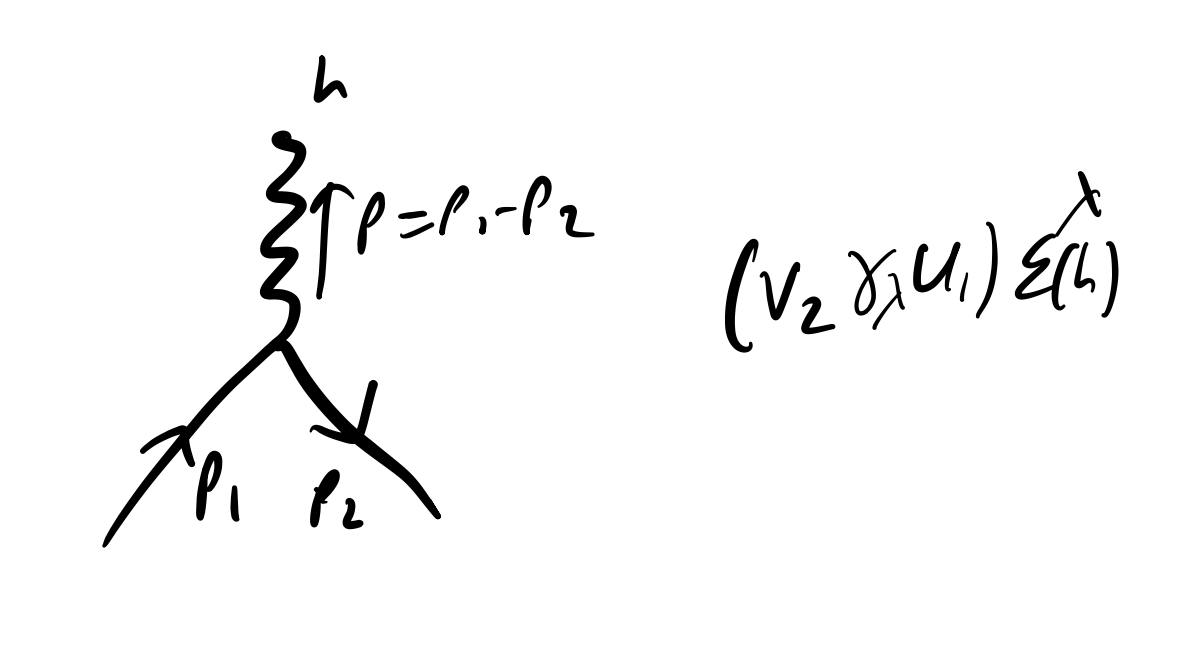
\includegraphics[scale=0.35]{Lectures/Images/lec15-wardidentities.png}
\end{center}

Wherein:
\begin{equation}
    (v_2\gamma_\lambda u_1)\e^{\lambda}_{(h)} \stackrel{\e^\lambda \propto p_1 + p_2}{=} v_2(\slashed{p}_2 + \slashed{p}_1)u_1 = 0.
\end{equation}

Thus we have found;
\begin{equation}
    \sigma = \int \frac{1}{2s}\abs{\mathcal{M}}^2 d\Pi_{\text{LIPS}} = \frac{e^6}{2s^4}\frac{1}{4}\Tr(\gamma_\lambda \slashed{p}_1 \gamma_{\lambda'}\slashed{p}_2)\int \Tr(J^{\nu\lambda}\slashed{p}_4J^{\lambda'}_{\sp\nu}\slashed{p}_3)d\Pi_{\text{LIPS}}
\end{equation}
and in this integral we will see the IR divergence arise! The rest is just tedious/simple calculations.